\chapter{Testcompass}


\section{Reflexión sobre el modelado}
Tras completar los ejercicios es posible reflexionar sobre las diferencias entre los dos enfoques de modelado mencionados durante la clase.

\textbf{Modelado del dominio:} Representa la lógica de negocio real del sistema, describiendo qué hace el sistema funcionalmente.

\textbf{Modelado para testing:} Se enfoca en la verificación del sistema, diseñando escenarios de prueba para cubrir todas las rutas posibles, incluyendo casos límite y errores. Describe cómo verificamos que el sistema funciona.

La diferencia principal: el modelado del dominio busca mostrar como funciona el sistema, mientras que el modelado para testing busca cobertura exhaustiva de comportamientos.

\section{Ejercicios}
A continuación se muestran los PNG de los modelos.

\begin{figure}[htbp]
    \centering
    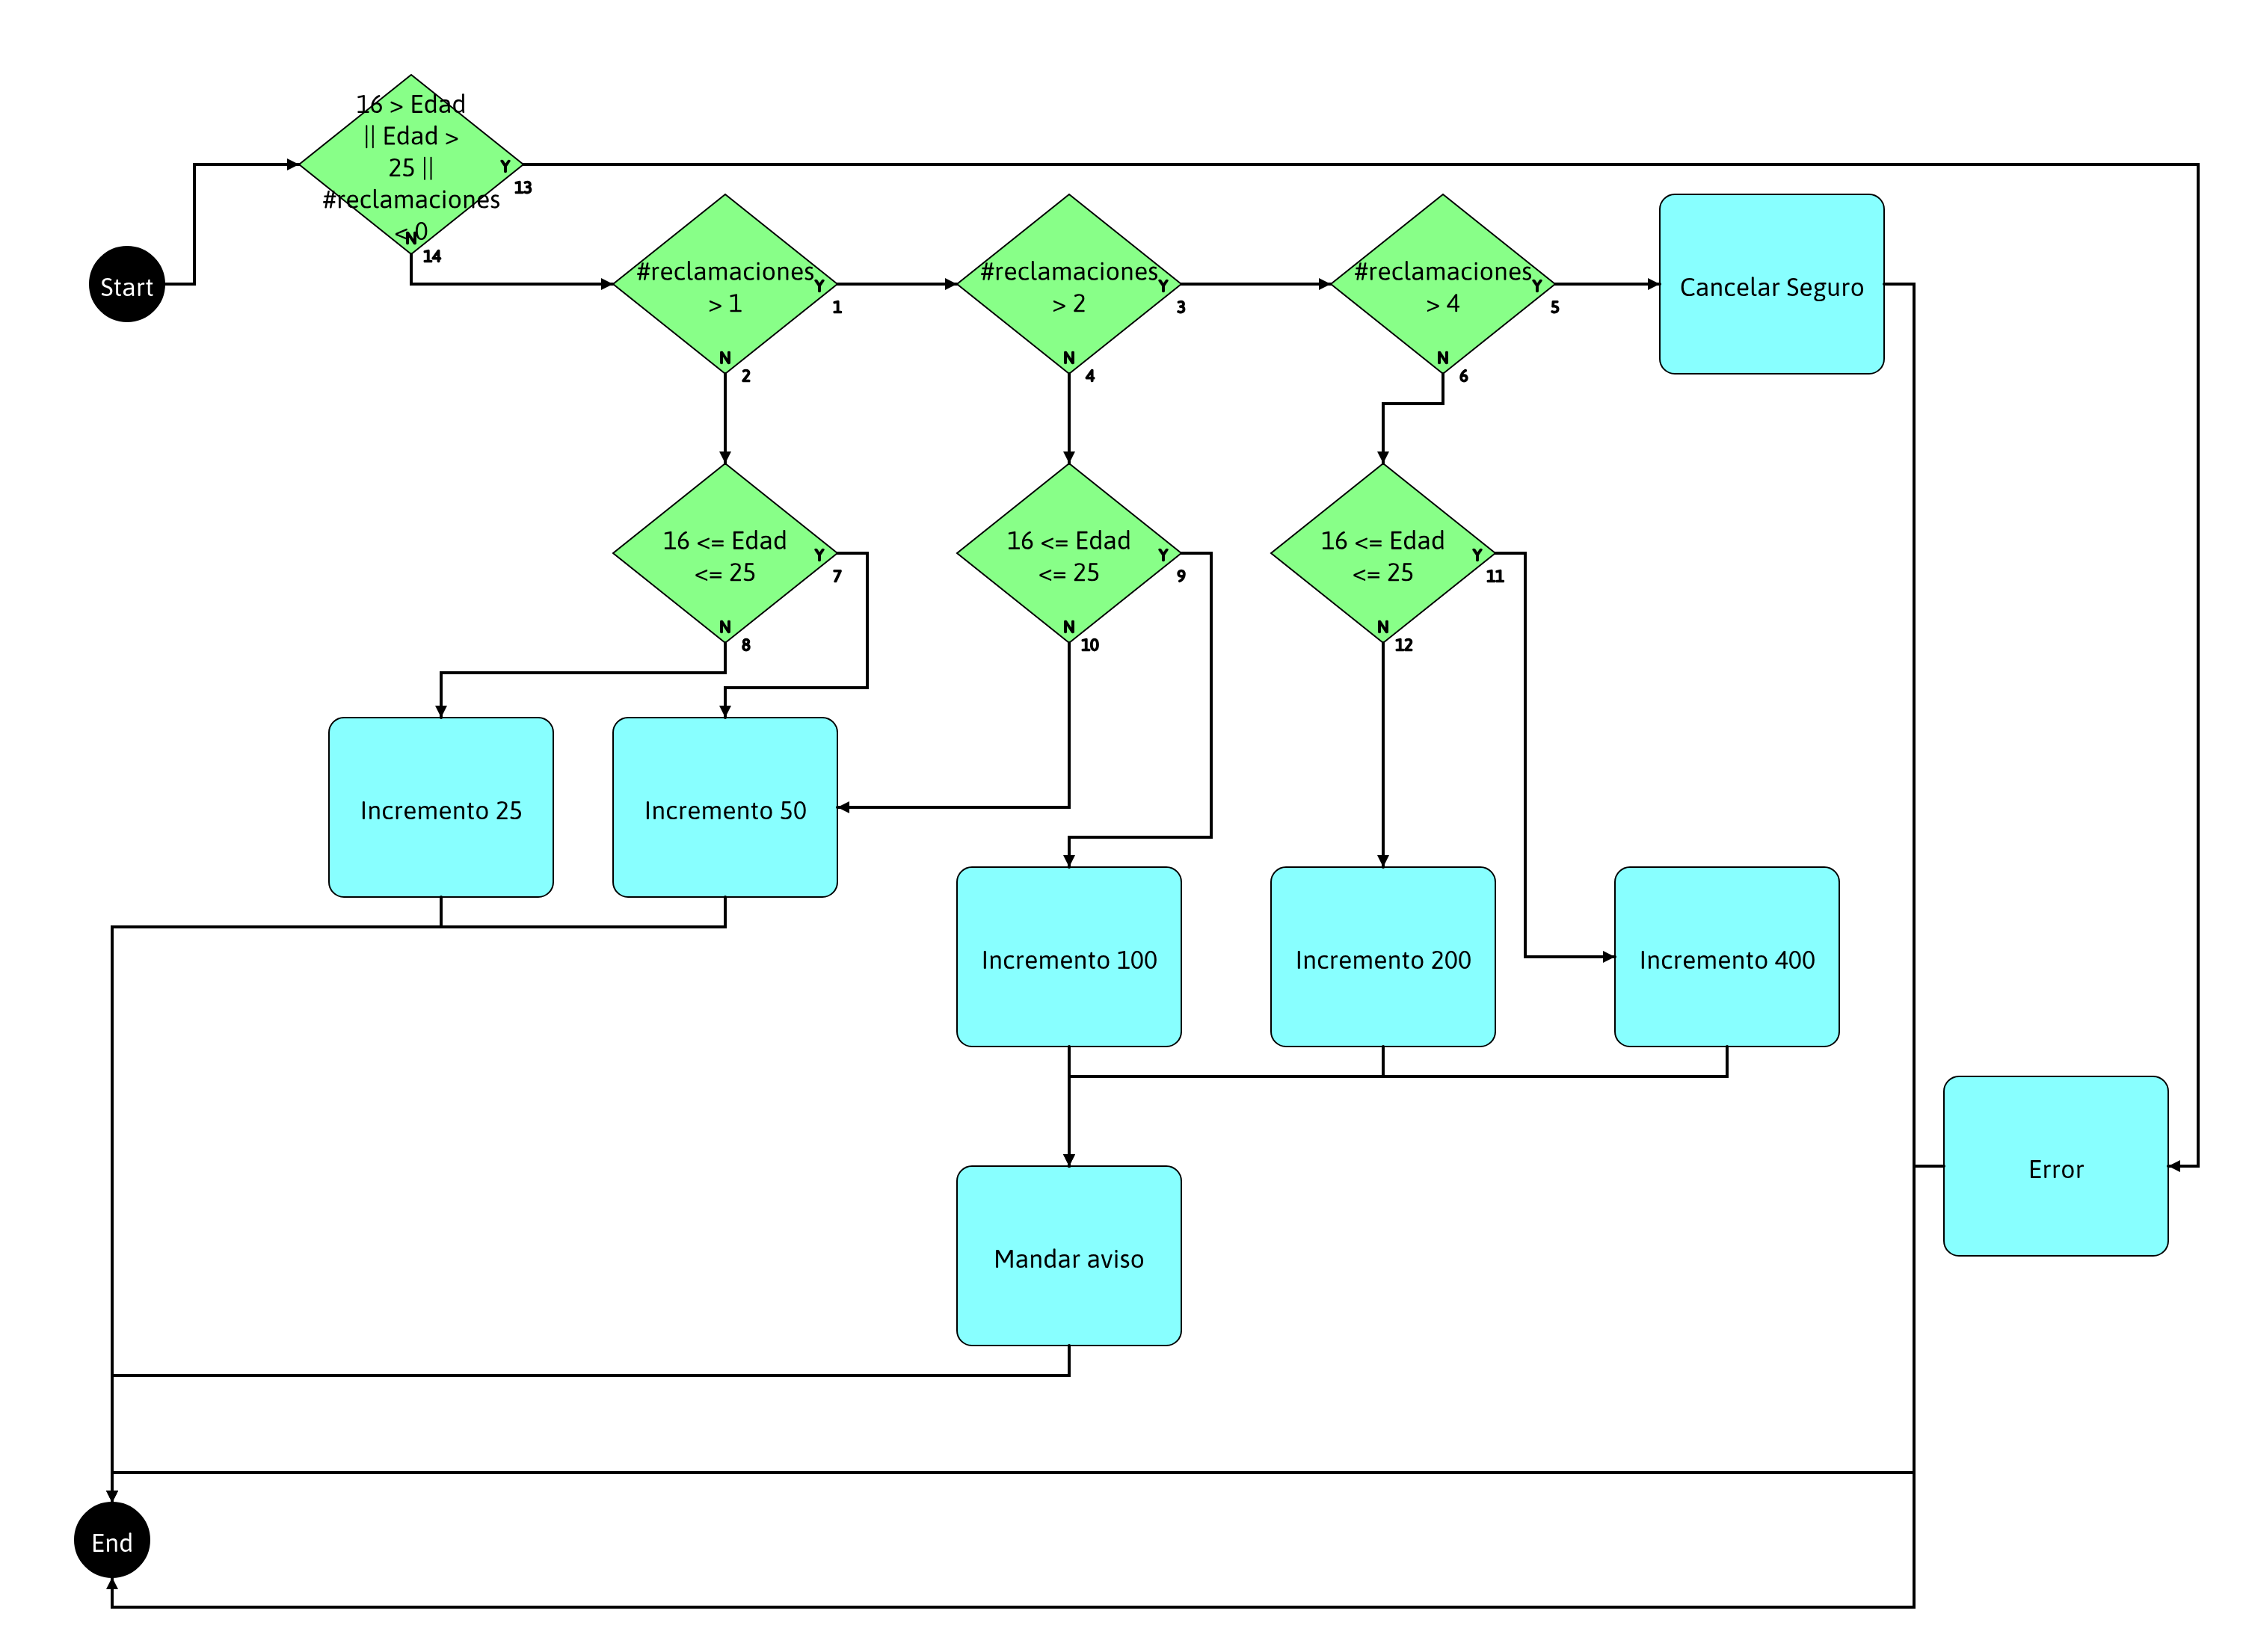
\includegraphics[width=0.95\columnwidth]{images/SeguroCoche.png}
    \caption{Ejercicio 1 - Seguro de coche}
    \label{fig:SeguroCoche}
\end{figure}

\begin{figure}[htbp]
    \centering
    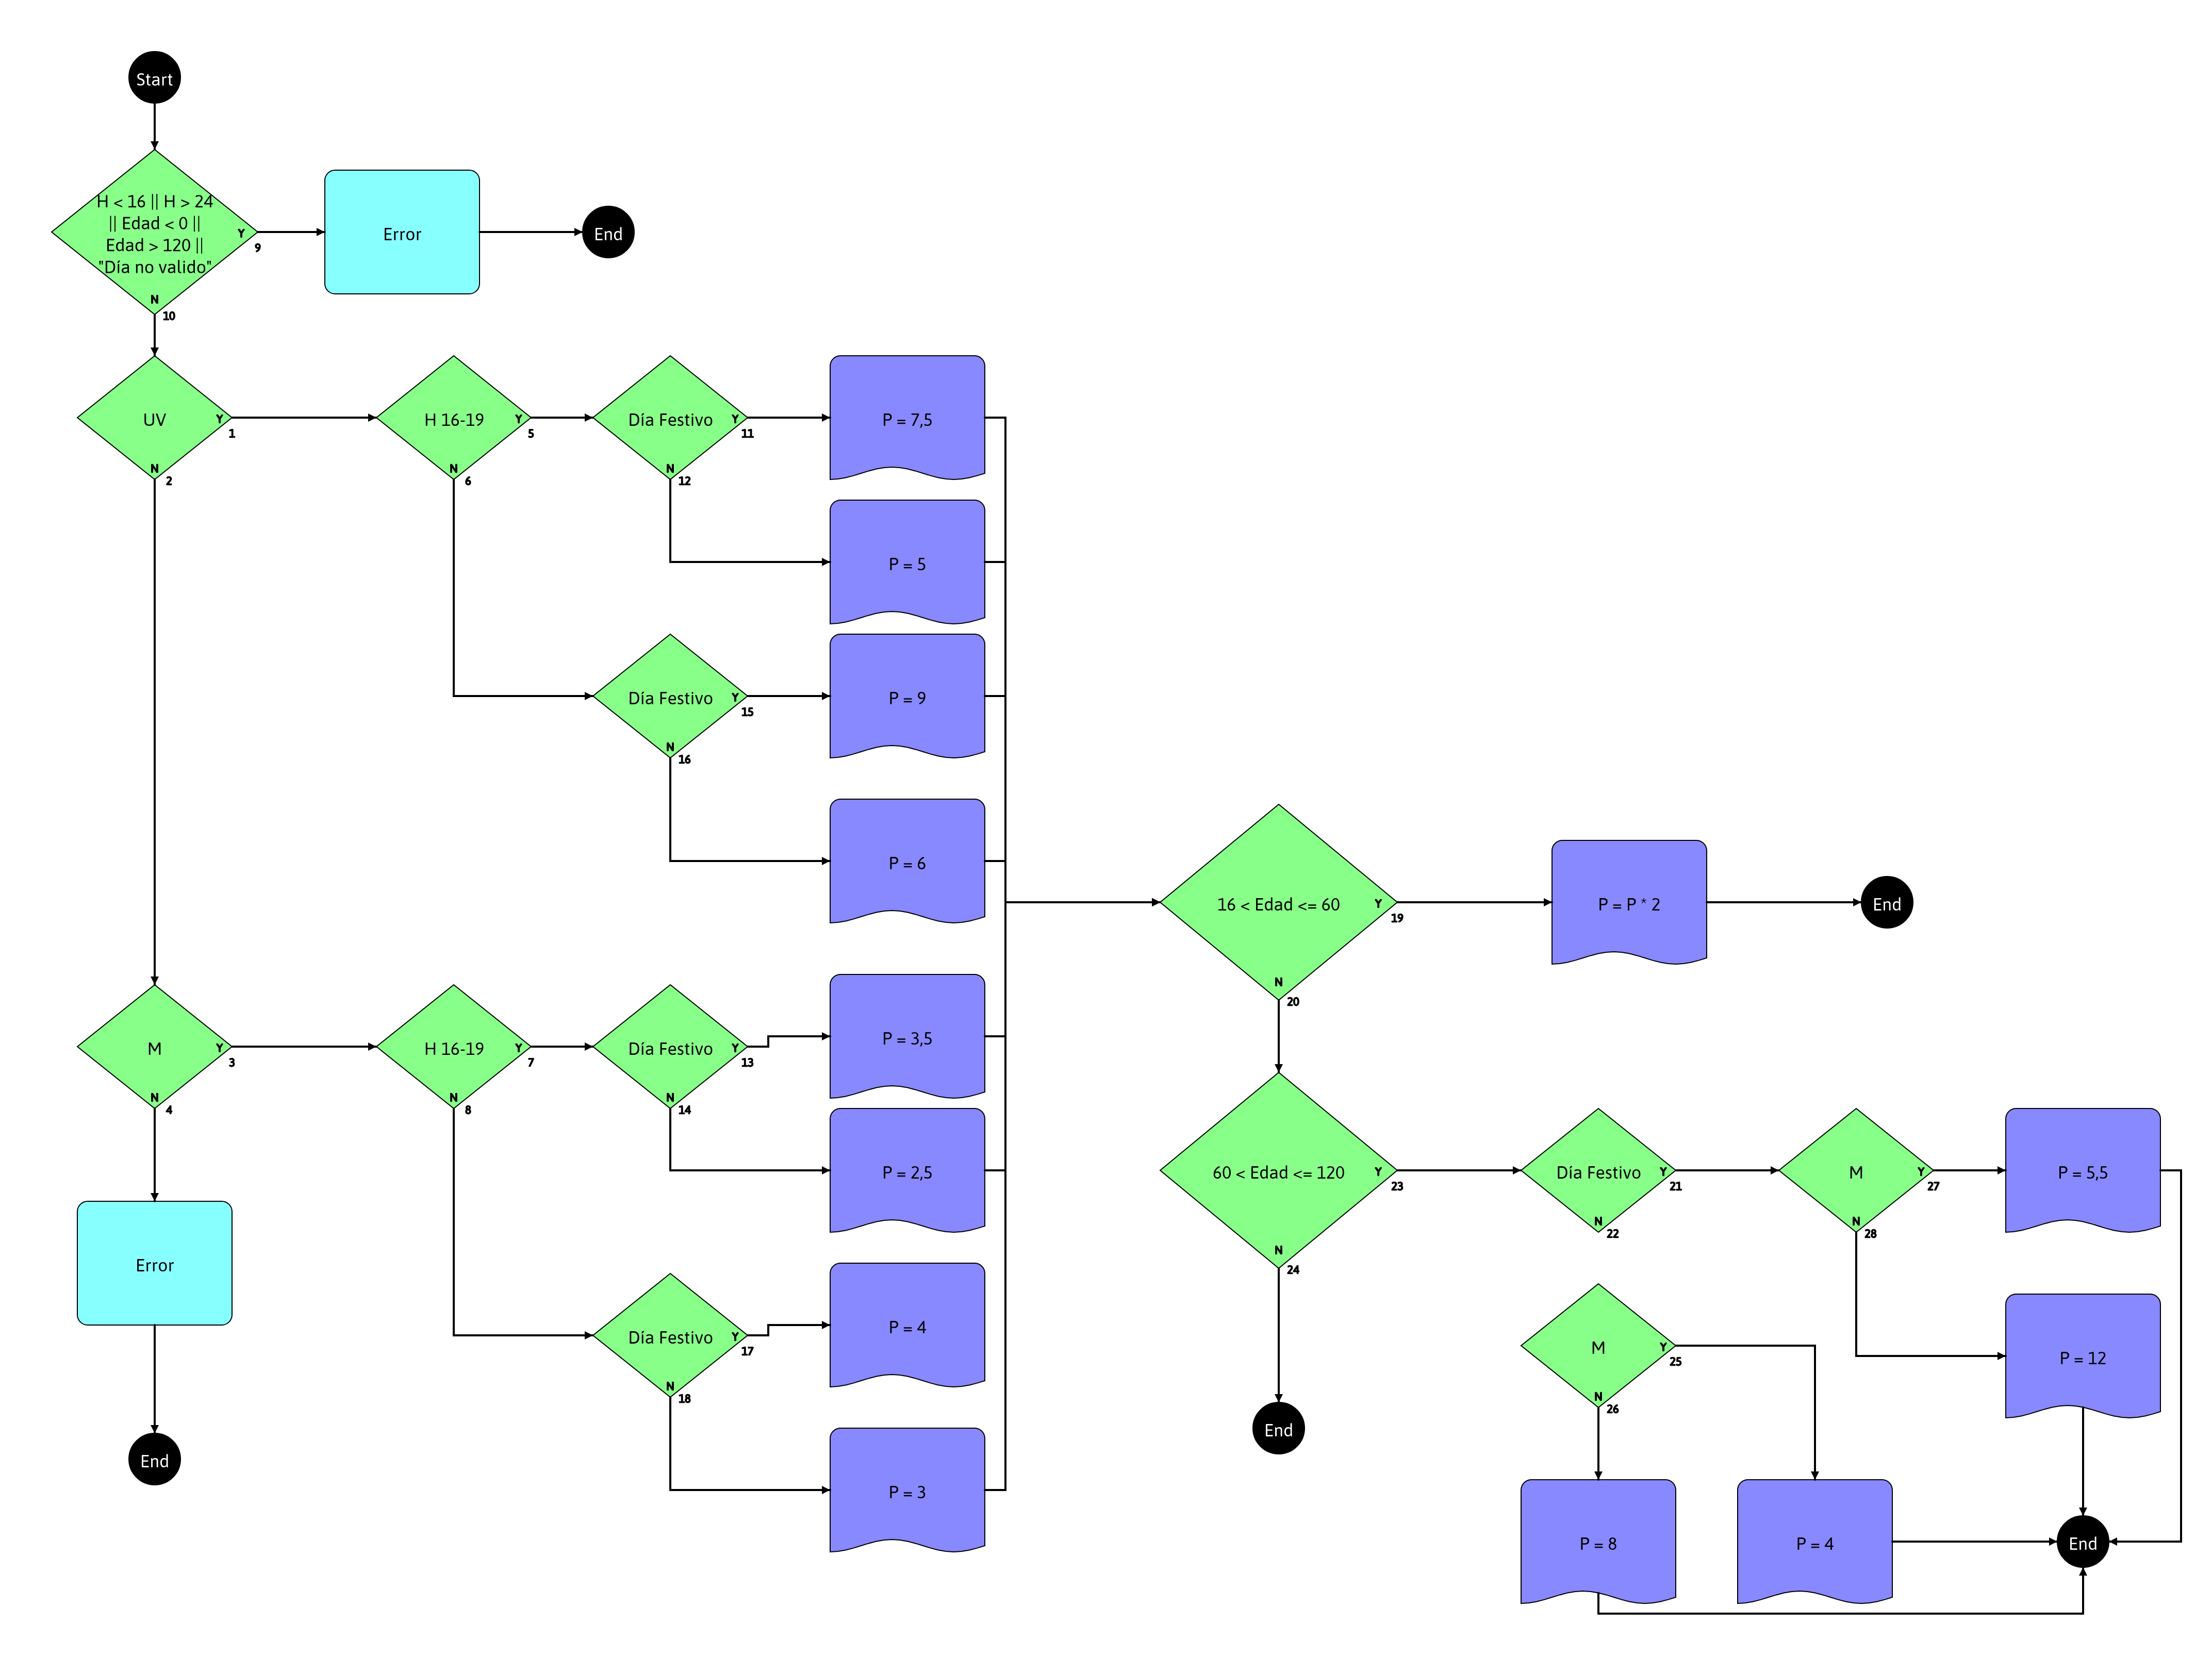
\includegraphics[width=0.95\columnwidth]{images/Piscina.png}
    \caption{Ejercicio 2 - Piscina}
    \label{fig:Piscina}
\end{figure}

\begin{figure}[htbp]
    \centering
    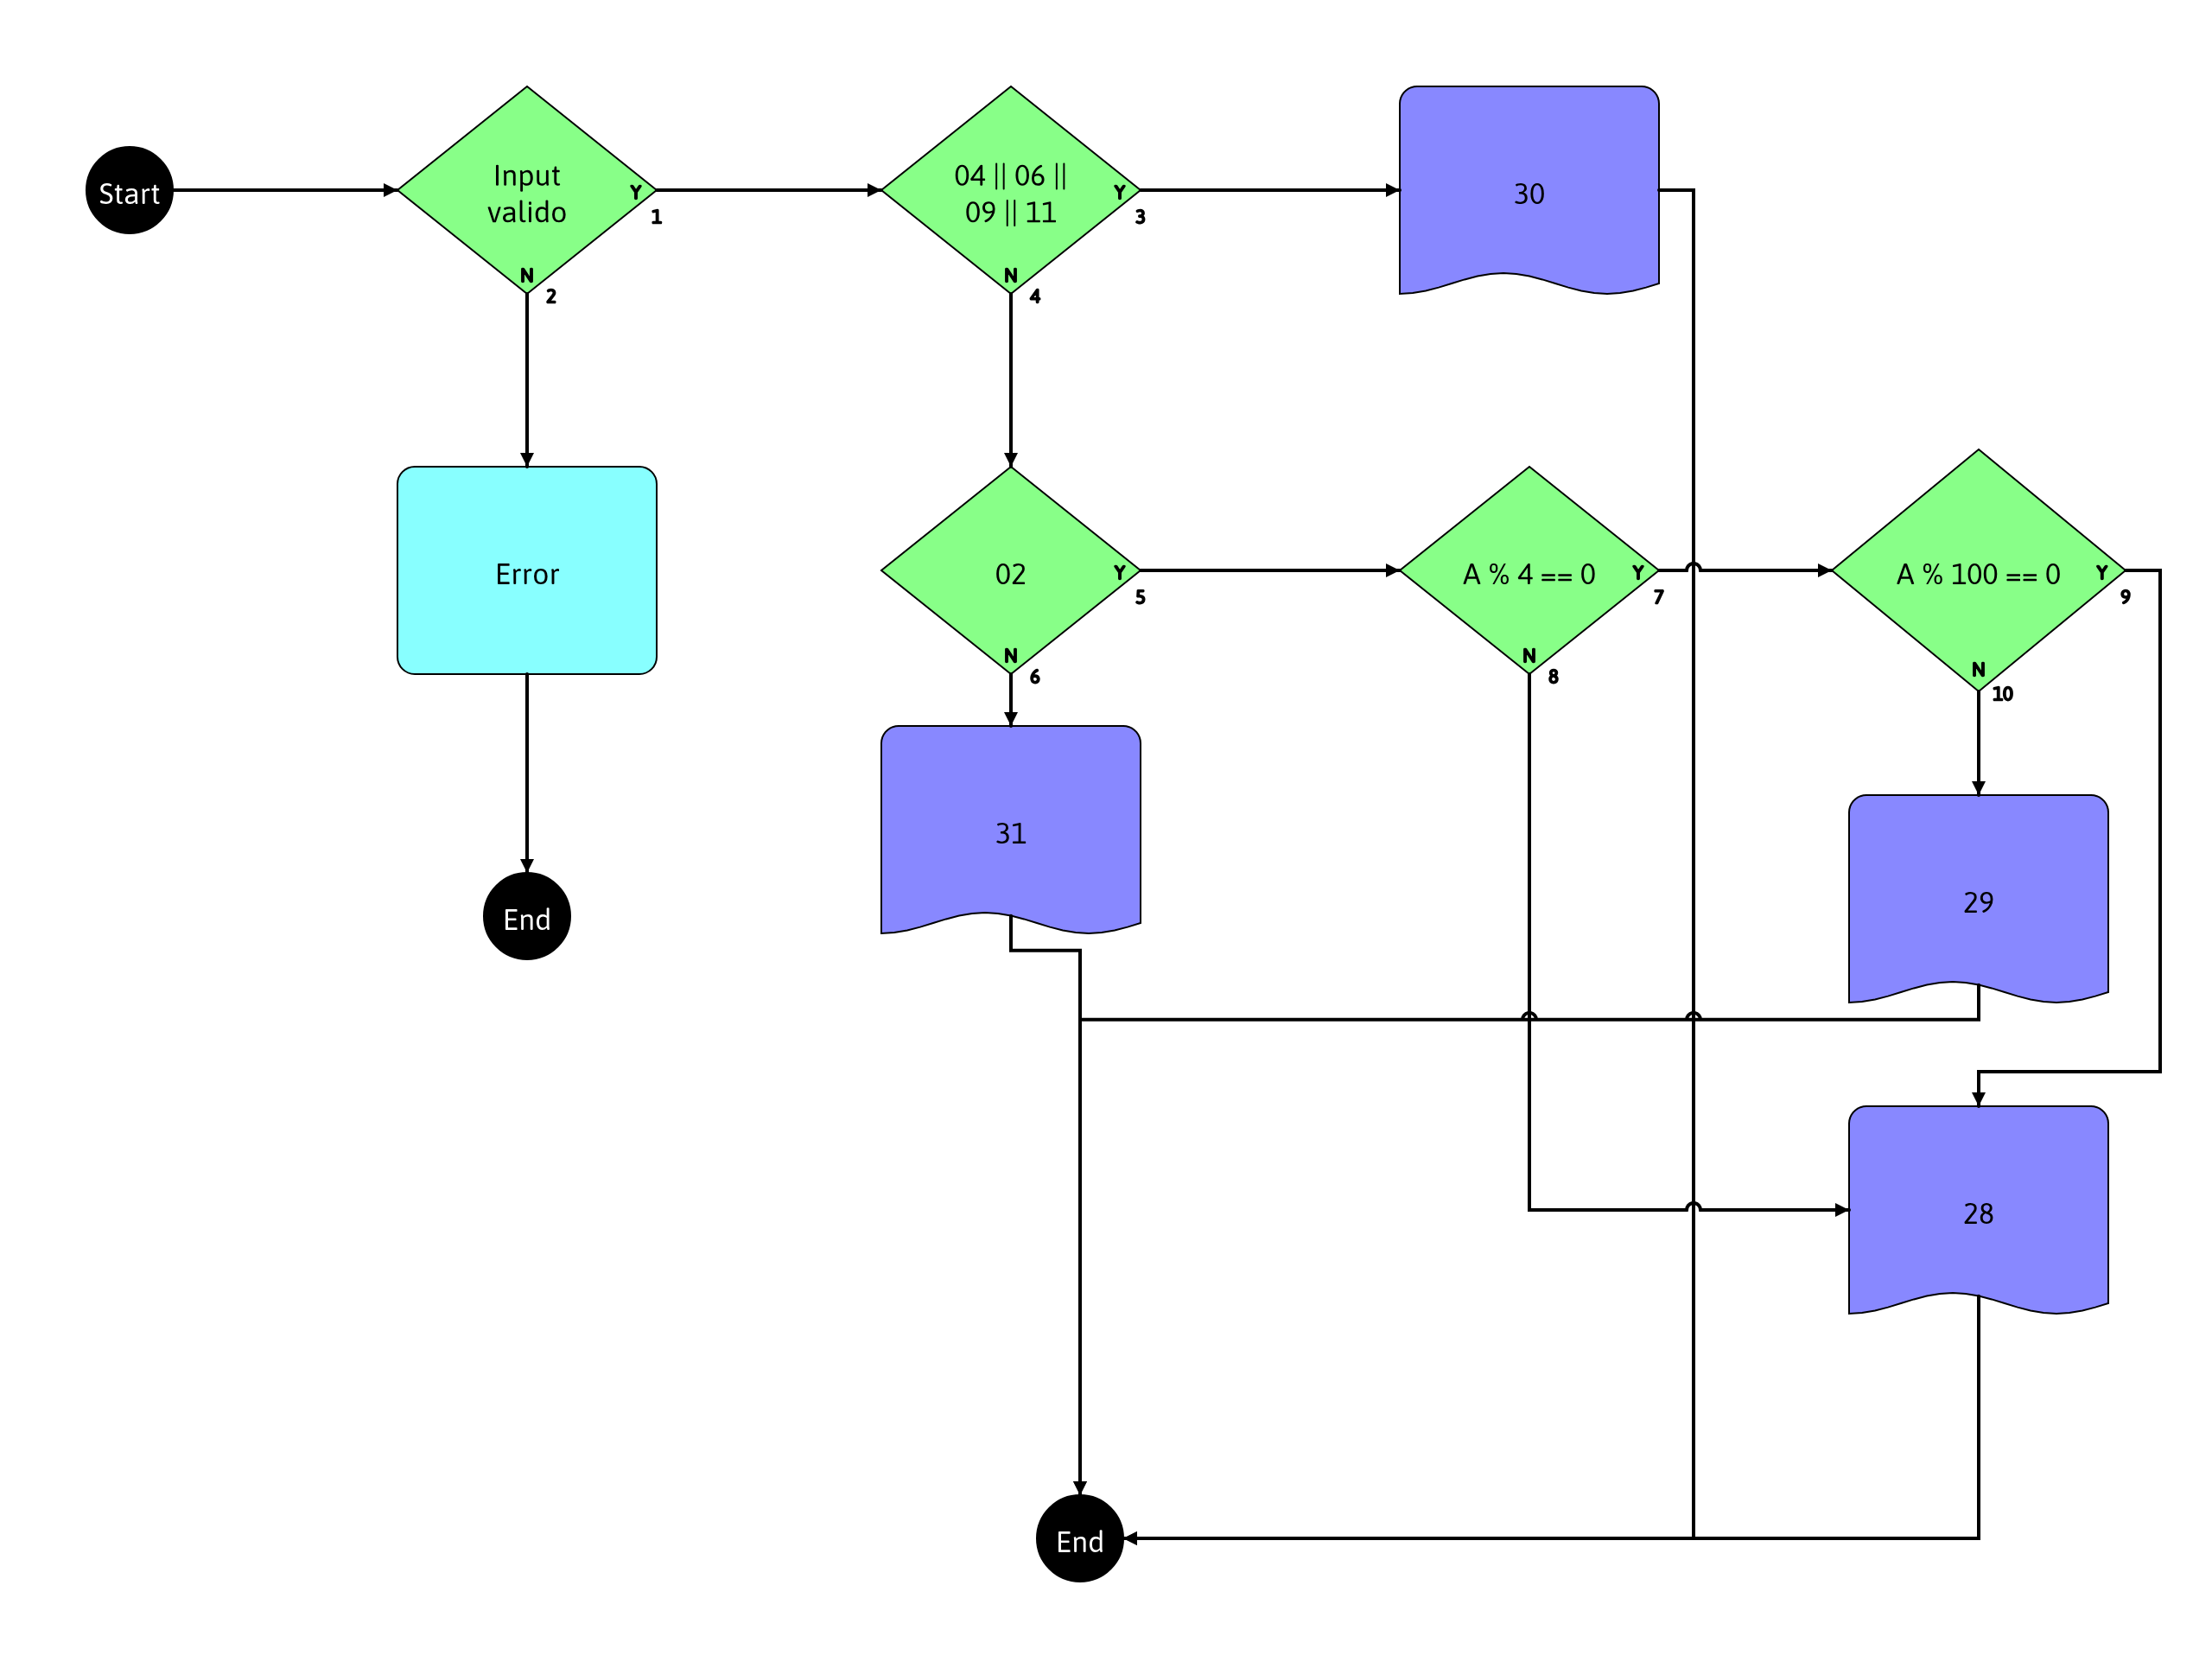
\includegraphics[width=0.95\columnwidth]{images/Bisiesto.png}
    \caption{Ejercicio 3 - Bisiesto}
    \label{fig:Bisiesto}
\end{figure}

\begin{figure}[htbp]
    \centering
    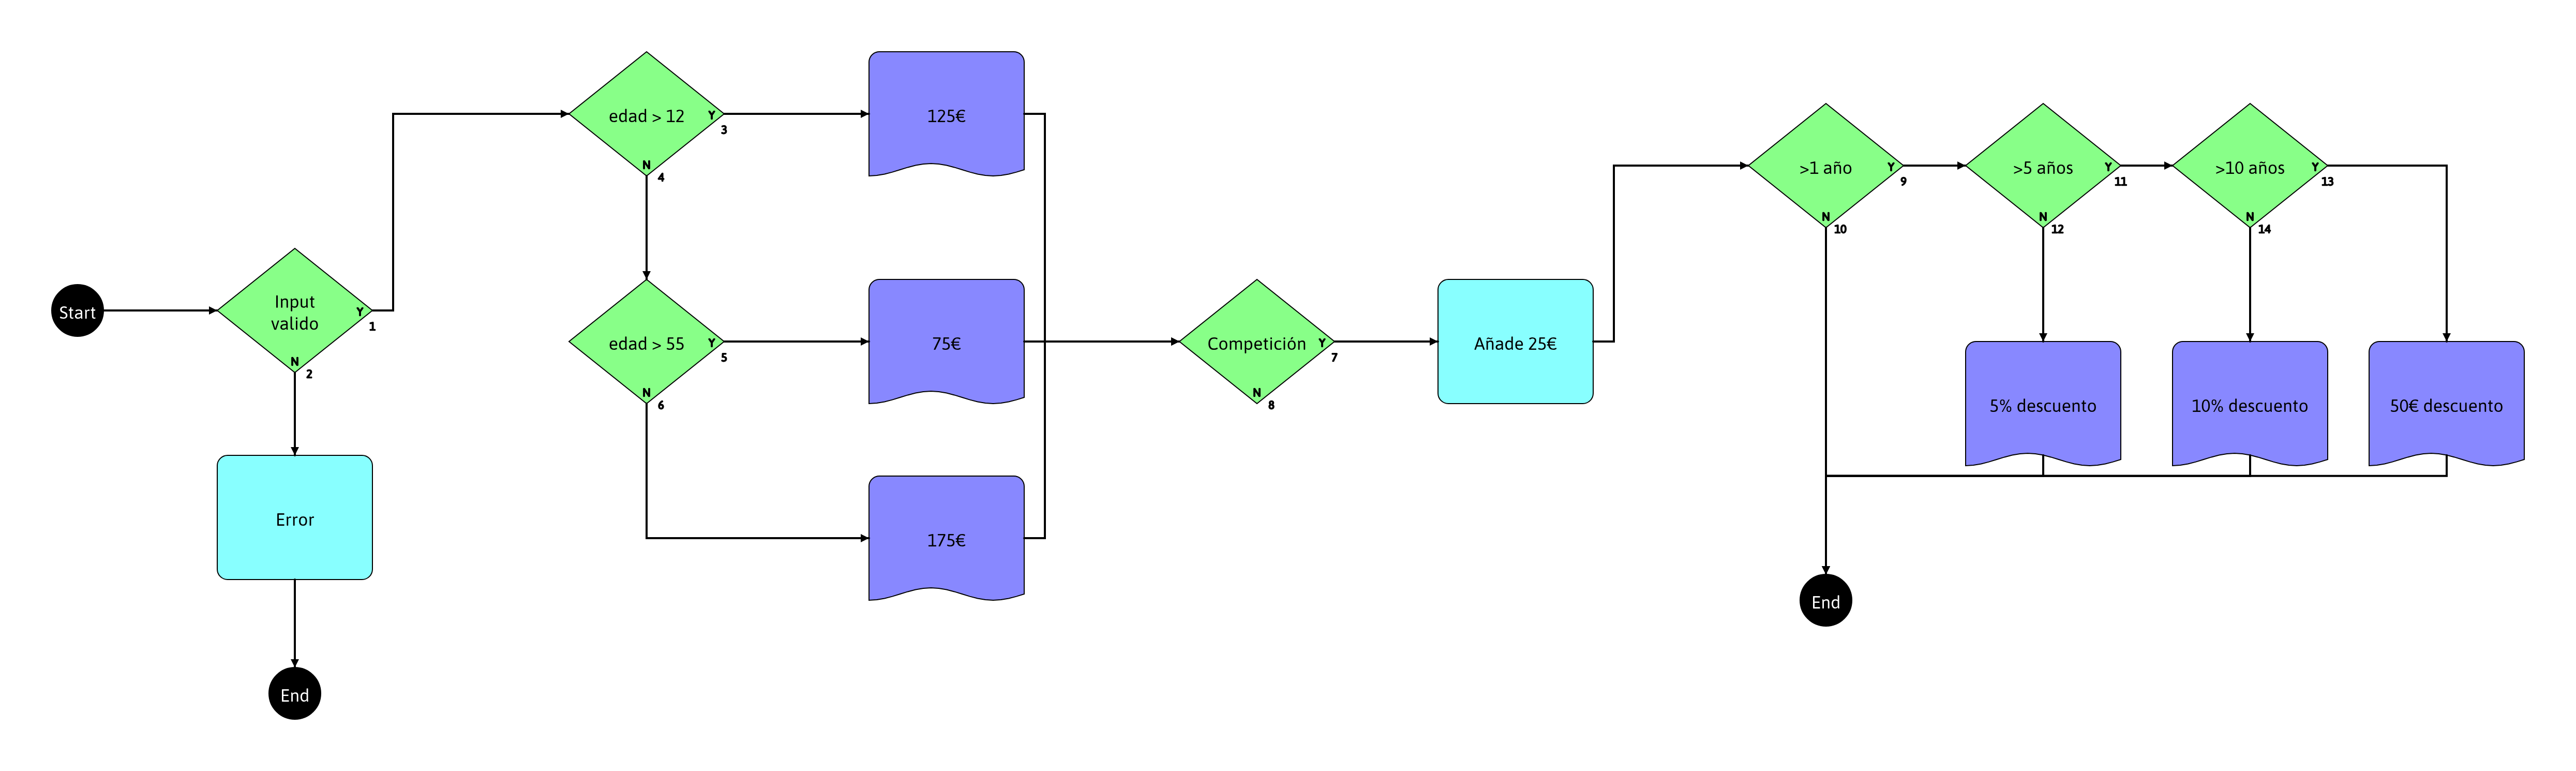
\includegraphics[width=0.95\columnwidth]{images/Football.png}
    \caption{Ejercicio 4 - Football}
    \label{fig:Football}
\end{figure}

\begin{figure}[htbp]
    \centering
    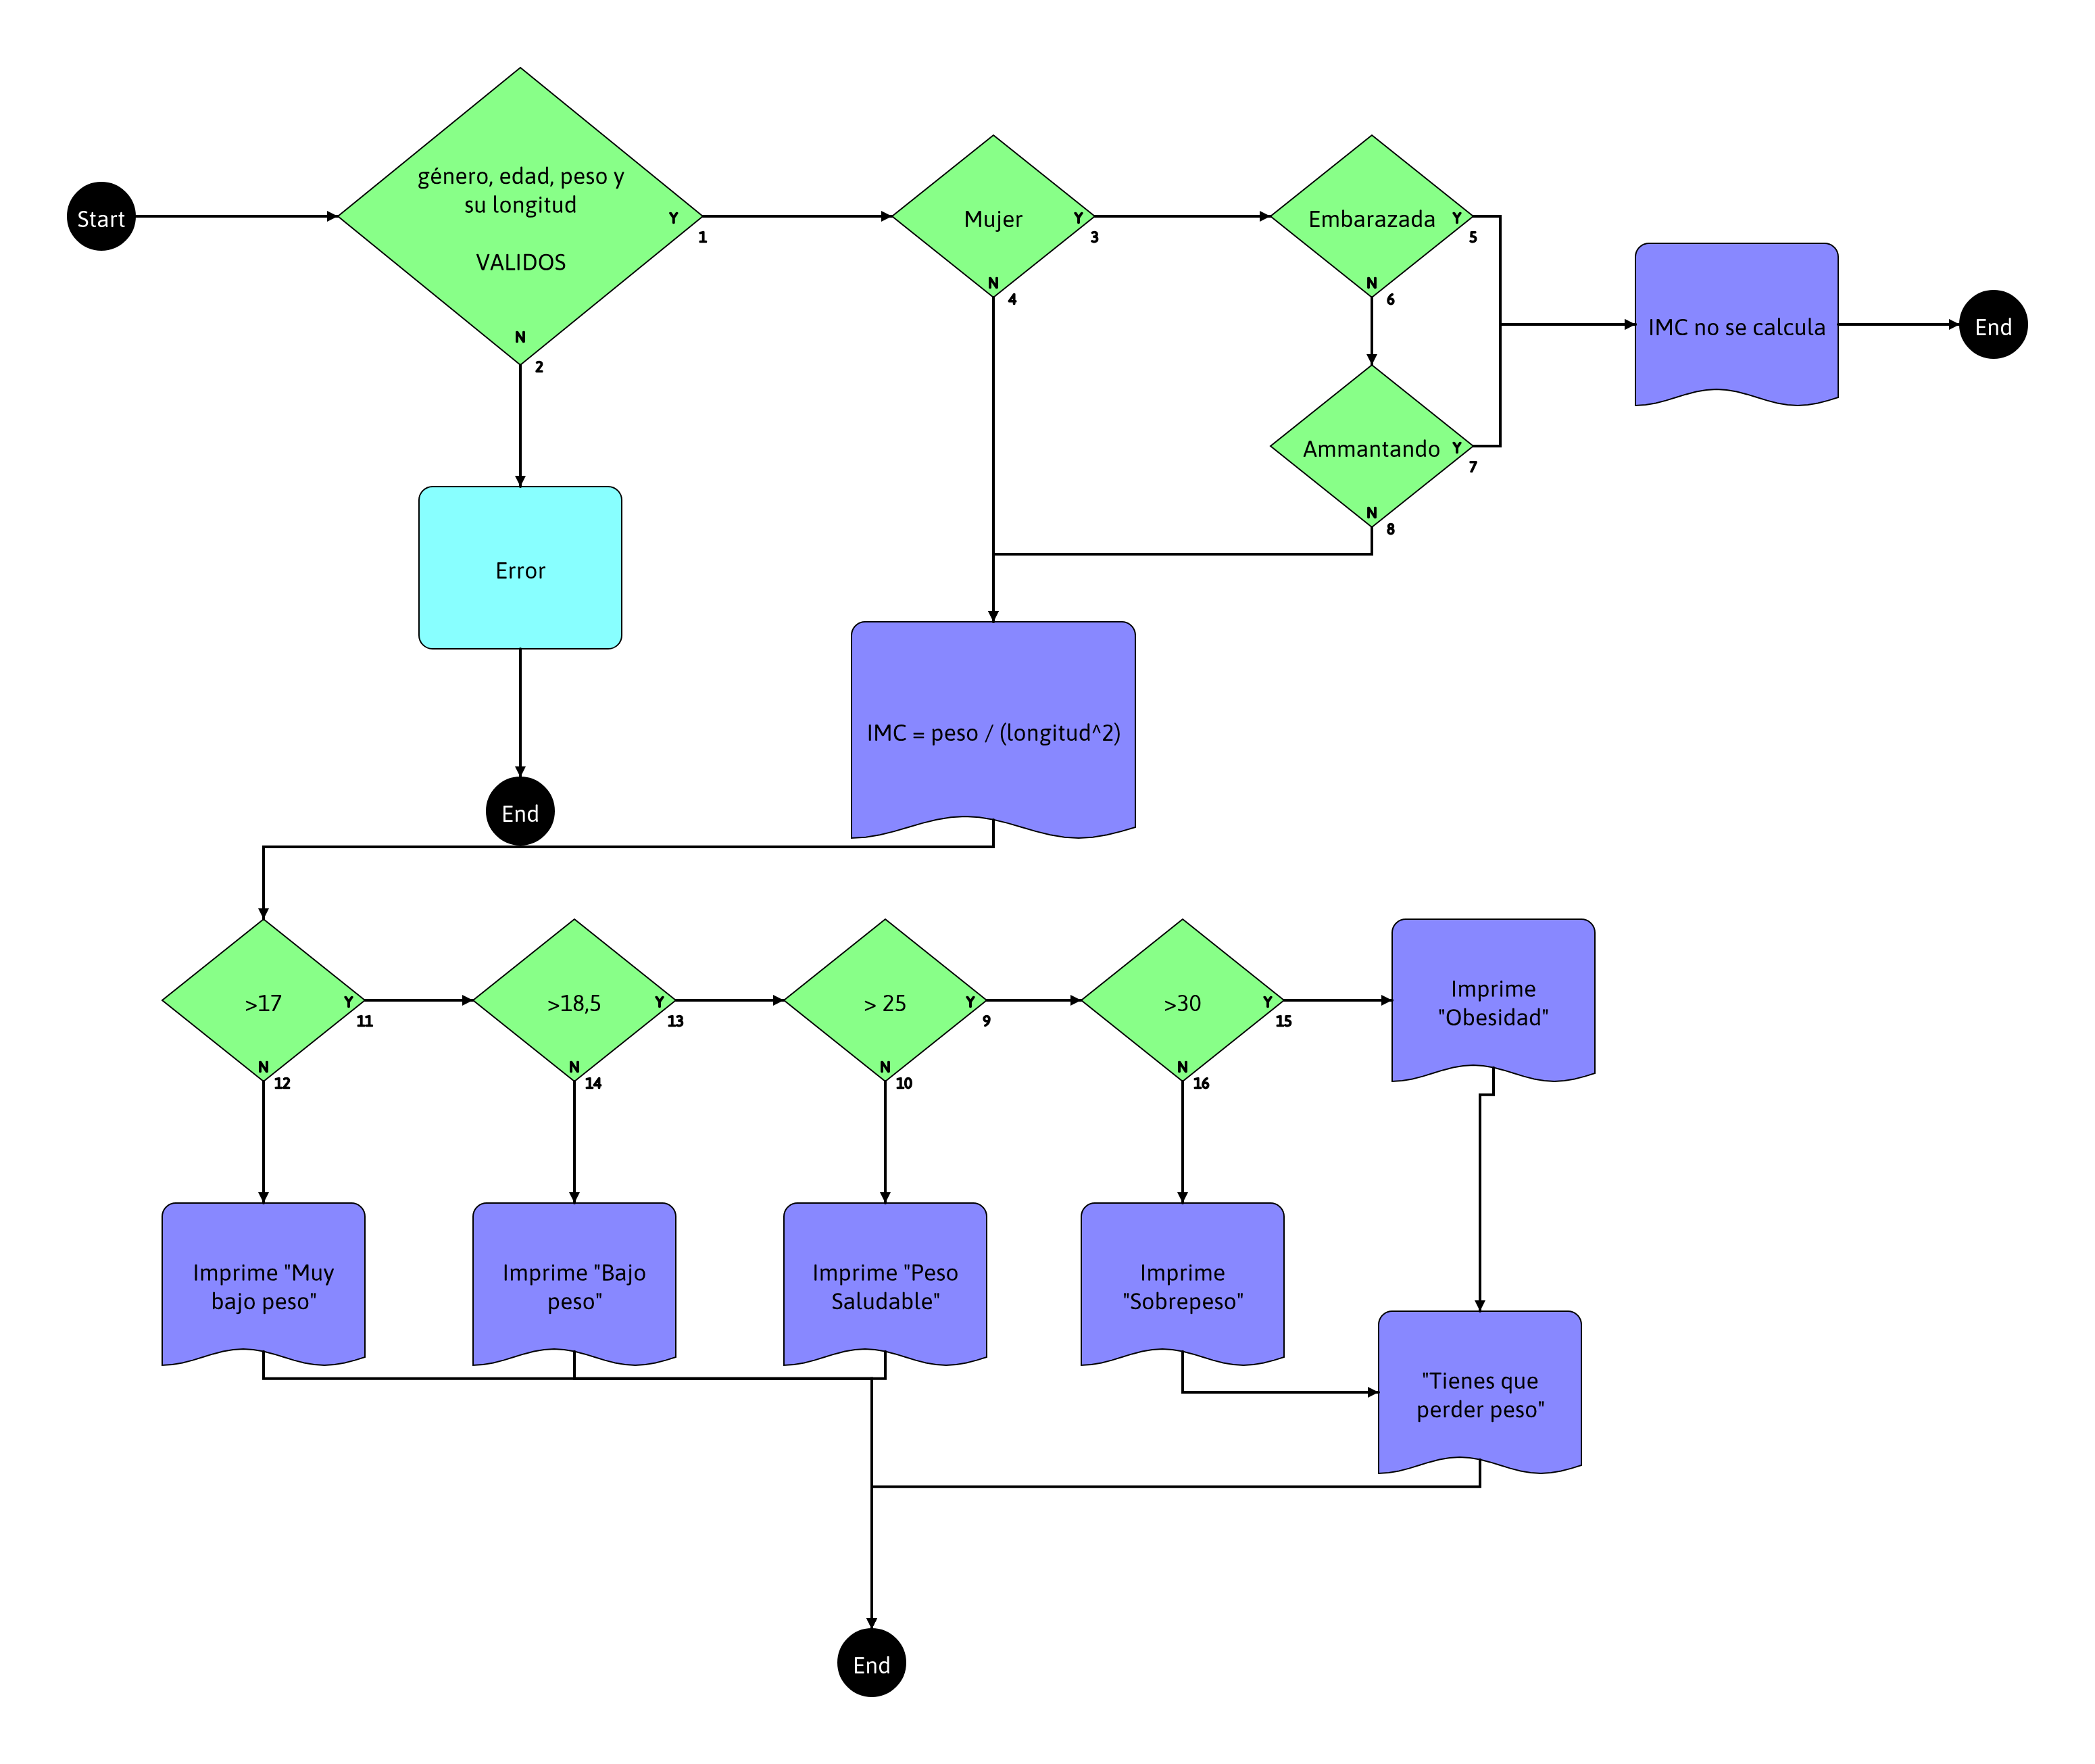
\includegraphics[width=0.95\columnwidth]{images/Calculadora.png}
    \caption{Ejercicio 5 - Calculadora IMC}
    \label{fig:Calculadora}
\end{figure}
